\section{Excision and applications}
We have found two general properties of singular homology: homotopy invariance and the long exact sequence of a pair. We also claimed that $H_\ast(X,A)$ ``depends only on $X-A$.'' You have to be careful about this. The following definition gives conditions that will capture the sense in which the relative homology of a pair $(X,A)$ depends only on the complement of $A$ in $X$. 
\begin{definition}
A triple $(X,A,U)$ where $U\subseteq A\subseteq X$, is \emph{excisive} if $\overline{U}\subseteq\mathrm{Int}(A)$. 
The inclusion $(X-U,A-U)\subseteq (X,A)$ is then called an {\em excision}.
\end{definition}

\begin{theorem}
An excision induces an isomorphism in homology,
\[
H_\ast(X-U,A-U)\xrightarrow{\cong}H_\ast(X,A)\,.
\]
\end{theorem}
So you can cut out closed bits of the interior of $A$ without changing the relative homology. The proof will take us a couple of days. Before we give applications, let me pose a different way to interpret the motto ``$H_*(X,A)$ depends only on $X-A$.'' Collapsing the subspace $A$ to a point gives us a map of pairs
\[
(X,A)\to(X/A,\ast)\,.
\]
When does this map induce an isomorphism in homology? Excision has the following consequence.
\begin{corollary} Assume that there is a subspace $B$ of $X$ such that 
{\em(1)} $\overline A\subseteq\mathrm{Int}B$ and 
{\em(2)} $A\to B$ is a deformation retract.
Then 
\[
H_*(X,A)\to H_*(X/A,*)
\]
is an isomorphism. 
\end{corollary}
\begin{proof} 
The diagram of pairs
\[
\xymatrix{
(X,A) \ar[d] \ar[r]^i & (X,B) \ar[d] & (X-A,B-A) \ar[d]^k \ar[l]_j \\
(X/A,\ast) \ar[r]^{\overline\imath} & (X/A,B/A) & 
(X/A-\ast,B/A-\ast) \ar[l]_{\overline\jmath} 
}\]
commutes. We want the left vertical to be a homology isomorphism, and
will show that the rest of the perimeter consists of homology isomorphisms.  
The map $k$ is a homeomorphism of pairs while $j$ is an excision by assumption
(1). The map $i$ induces an isomorphism in homology by assumption (2),
the long exact sequences, and the five-lemma.
Since $I$ is a compact Hausdorff space, the map $B\times I\to B/A\times I$
is again a quotient map, so the deformation $B\times I\to B$, that restricts
to the constant deformation on $A$, descends to show that $\ast\to B/A$ 
is a deformation retract. So the map $\overline\imath$ 
is also a homology isomorphism. 
Finally, $\overline\ast\subseteq\mathrm{Int}(B/A)$ in $X/A$, by definition
of the quotient topology, so $\overline\jmath$ induces an isomorphism by
excision. 
\end{proof}

Now what are some consequences? For a start, we'll finally get around
to computing the homology of the sphere. 
It happens simultaneously with a computation of 
$ H^\ast(D^n,S^{n-1})$. (Note that $S^{-1}=\varnothing$.)
To describe generators, for each $n\geq0$ pick a homeomorphism
\[
(\Delta^n,\partial\Delta^n)\to(D^n,S^{n-1})\,,
\]
and write 
\[
\iota_n\in S_n(D^n,S^{n-1})
\]
for the corresponding relative $n$-chain.
\begin{prop} Let $\ast\in S^{n-1}$ be any point (for $n>0$). 
	 \begin{equation*}
	 H_q(S^n)=\begin{cases}
\Z = \langle[\partial\iota_{n+1}]\rangle & \hbox{if}\quad q=n>0 \\ 
\Z = \langle[c^0_\ast]\rangle & \hbox{if}\quad q=0,n>0\\ 
\Z\oplus\Z = \langle[c^0_\ast],[\partial\iota_1]\rangle & \hbox{if}\quad  q=n=0 \\
0 & \hbox{otherwise} \end{cases}
	\end{equation*}

	\item \begin{equation*}
	 H_q(D^n,S^{n-1}) = \begin{cases}
	\Z=\langle [\iota_n]\rangle & \hbox{if}\quad q=n\\
	0 & \hbox{otherwise}
	\end{cases}
	\end{equation*}
\end{prop}

\begin{proof}
The division into cases for $H_q(S^n)$ can be eased by employing reduced 
homology. Then the claim is merely that for $n\geq0$
\[
\widetilde H_q(S^{n-1})=
\begin{cases}\ZZ & \hbox{if}\quad q=n-1 \\ 
0 & \hbox{if}\quad q\neq n-1\end{cases}
\]
and the map 
\[
\partial:H_q(D^n,S^{n-1})\to \widetilde H_{q-1}(S^{n-1})
\]
is an isomorphism.  The second statement follows from the long exact sequence
in reduced homology together with the fact that $\widetilde H_*(D^n)=0$ 
since $D^n$ is contractible. The first uses induction and the pair of
isomorphisms
\[
\widetilde H_{q-1}(S^{n-1}) \xleftarrow{\cong}H_q(D^n,S^{n-1})
\xrightarrow{\cong}H_q(D^n/S^{n-1},\ast)
\]
since $D^n/S^{n-1}\cong S^n$. The right hand arrow is an isomorphism 
since $S^{n-1}$ is a deformation retract of a neighborhood in $D^n$.
\end{proof}

Why should you care about this complicated homology calculation?
\begin{corollary}
If $m\neq n$, then $S^m$ and $S^n$ are not homotopy equivalent.
\end{corollary}
\begin{proof}
Their homology groups are not isomorphic.
\end{proof}
\begin{corollary}
If $m\neq n$, then $\mathbf{R}^m$ and $\mathbf{R}^n$ are not homeomorphic.
\end{corollary}
\begin{proof}
If $m$ or $n$ is zero, this is clear, so 
let $m,n>0$. Assume we have a homeomorphism $f:\mathbf{R}^m\to \mathbf{R}^n$. This restricts to a homeomorphism $\mathbf{R}^m-\{0\}\to \mathbf{R}^n-\{0\}$.
But these are homotopy equivalent to spheres, of different dimension.
\end{proof}
\begin{theorem}[Brouwer fixed-point theorem]
If $f:D^n\to D^n$ is continuous, 
then there is some point $x\in D^n$ such that $f(x)=x$.
\end{theorem}
\begin{proof}
Suppose not. Then you can draw a ray from $f(x)$ through $x$. It meets the boundary of $D^n$ at a point $g(x)\in S^{n-1}$. Check that $g$ is continuous. If $x$ is on the boundary, then $x=g(x)$, so $g$ is a null-homotopy of the identity map on $S^{n-1}$. This is inconsistent with our computation because the identity map induces the identity map on $\widetilde H_{n-1}(S^{n-1})\cong\ZZ$.
\end{proof}

\begin{center}
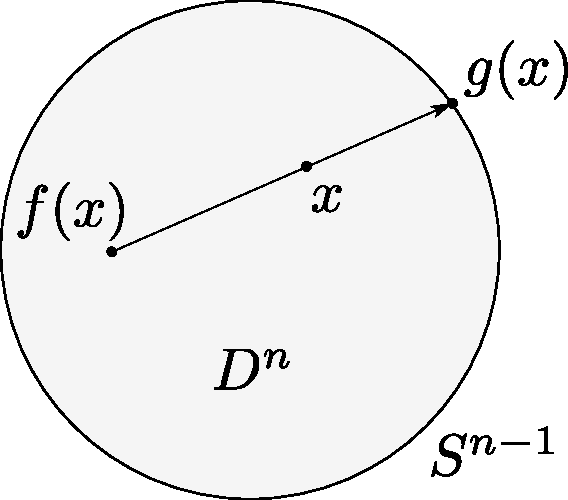
\includegraphics[width=3in]{905/Figures/10-Brouwer-FPT.pdf}
\end{center}


Our computation of the homology of a sphere also implies that there are many non-homotopic self-maps of $S^n$, for any $n\geq1$. We will distinguish them by means of the ``degree'': A map $f:S^n\to S^n$ induces an endomorphism of the infinite cyclic group $H_n(S^n)$. Any endomorphism of an infinite cyclic group is given by multiplication by an integer. This integer is well defined (independent of a choice of basis), and any integer occurs. Thus $\mathrm{End}(\ZZ)=\ZZ_\times$, the monoid of integers under multiplication. The homotopy classes of self-maps of $S^n$ also form a monoid, under composition, and: 
\begin{theorem}
Let $n\geq 1$. The degree map provides us with a surjective monoid homomorphism
\[
\mathrm{deg}:[S^n,S^n]\to \Z_\times\,.
\]
\end{theorem}
\begin{proof}
Degree is multiplicative by functoriality of homology.

Construction of a map of degree $k$: If $n=1$, this is just the winding number; an example is given by regardeing $S^1$ as unit complex numbers and sending $z$ to $z^k$. The proof that this has degree $k$ is an exercise. 

Suppose we've constructed a map $f_k:S^{n-1}\to S^{n-1}$ of degree $k$. 
Extend it to a map $\overline f_k:D^n\to D^n$ by defining 
$\overline f_k(tx)=tf_k(x)$ for $t\in[0,1]$. We may then collapse the sphere
to a point and identify the quotient with $S^n$. This gives us a new map
$g_k:S^n\to S^n$ making the diagram below commute.
	\begin{equation*}
	\xymatrix{ H_{n-1}(S^{n-1})\ar[d]^{f_{k*}} & \ar[l] H_n(D^n,S^{n-1})\ar[r]\ar[d] & H_n(S^n) \ar[d]^{g_{k*}}\\
	 H_{n-1}(S^{n-1}) & \ar[l] H_n(D^n,S^{n-1})\ar[r] & H_n(S^n)}
	\end{equation*}
The horizontal maps are isomorphisms, so $\deg g_k=k$ as well.
\end{proof}

We will see (in 18.906) that this map is in fact an isomorphism. 

